\section{Process Perspective}

%A description and illustration of:

\subsection{Team work}

%How do you interact as developers? 
%How is the team organized?
%Applied development process and tools supporting it
%For example, how did you use issues, Kanban boards, etc. to organize open tasks
%Applied branching strategy.

\subsubsection{Team organization}

Our project group has embraced a Scrum-like approach, working without a designated leader or specific areas of responsibility. We have integrated various elements from the Scrum framework into our week-to-week project work. We have prioritized meeting physically and working together, and have done so twice a week. During these meetings, we have conducted daily stand-up sessions to discuss progress, align our activities, and coordinate tasks. The remaining time was dedicated to project work, where team members collaborated either in pairs or individually. This flexible approach allowed us to adapt our working arrangements based on the tasks at hand and the preferences of team members.

\subsubsection{Collaboration and communication tools}

We have used \textit{Microsoft Teams} as the primary channel of day-to-day online communication. In addition, we used \textit{Notion} as a shared space for note-taking and organizing links to relevant resources, see Figure \ref{fig:notion}. 

\begin{figure}[H]
    \centering
    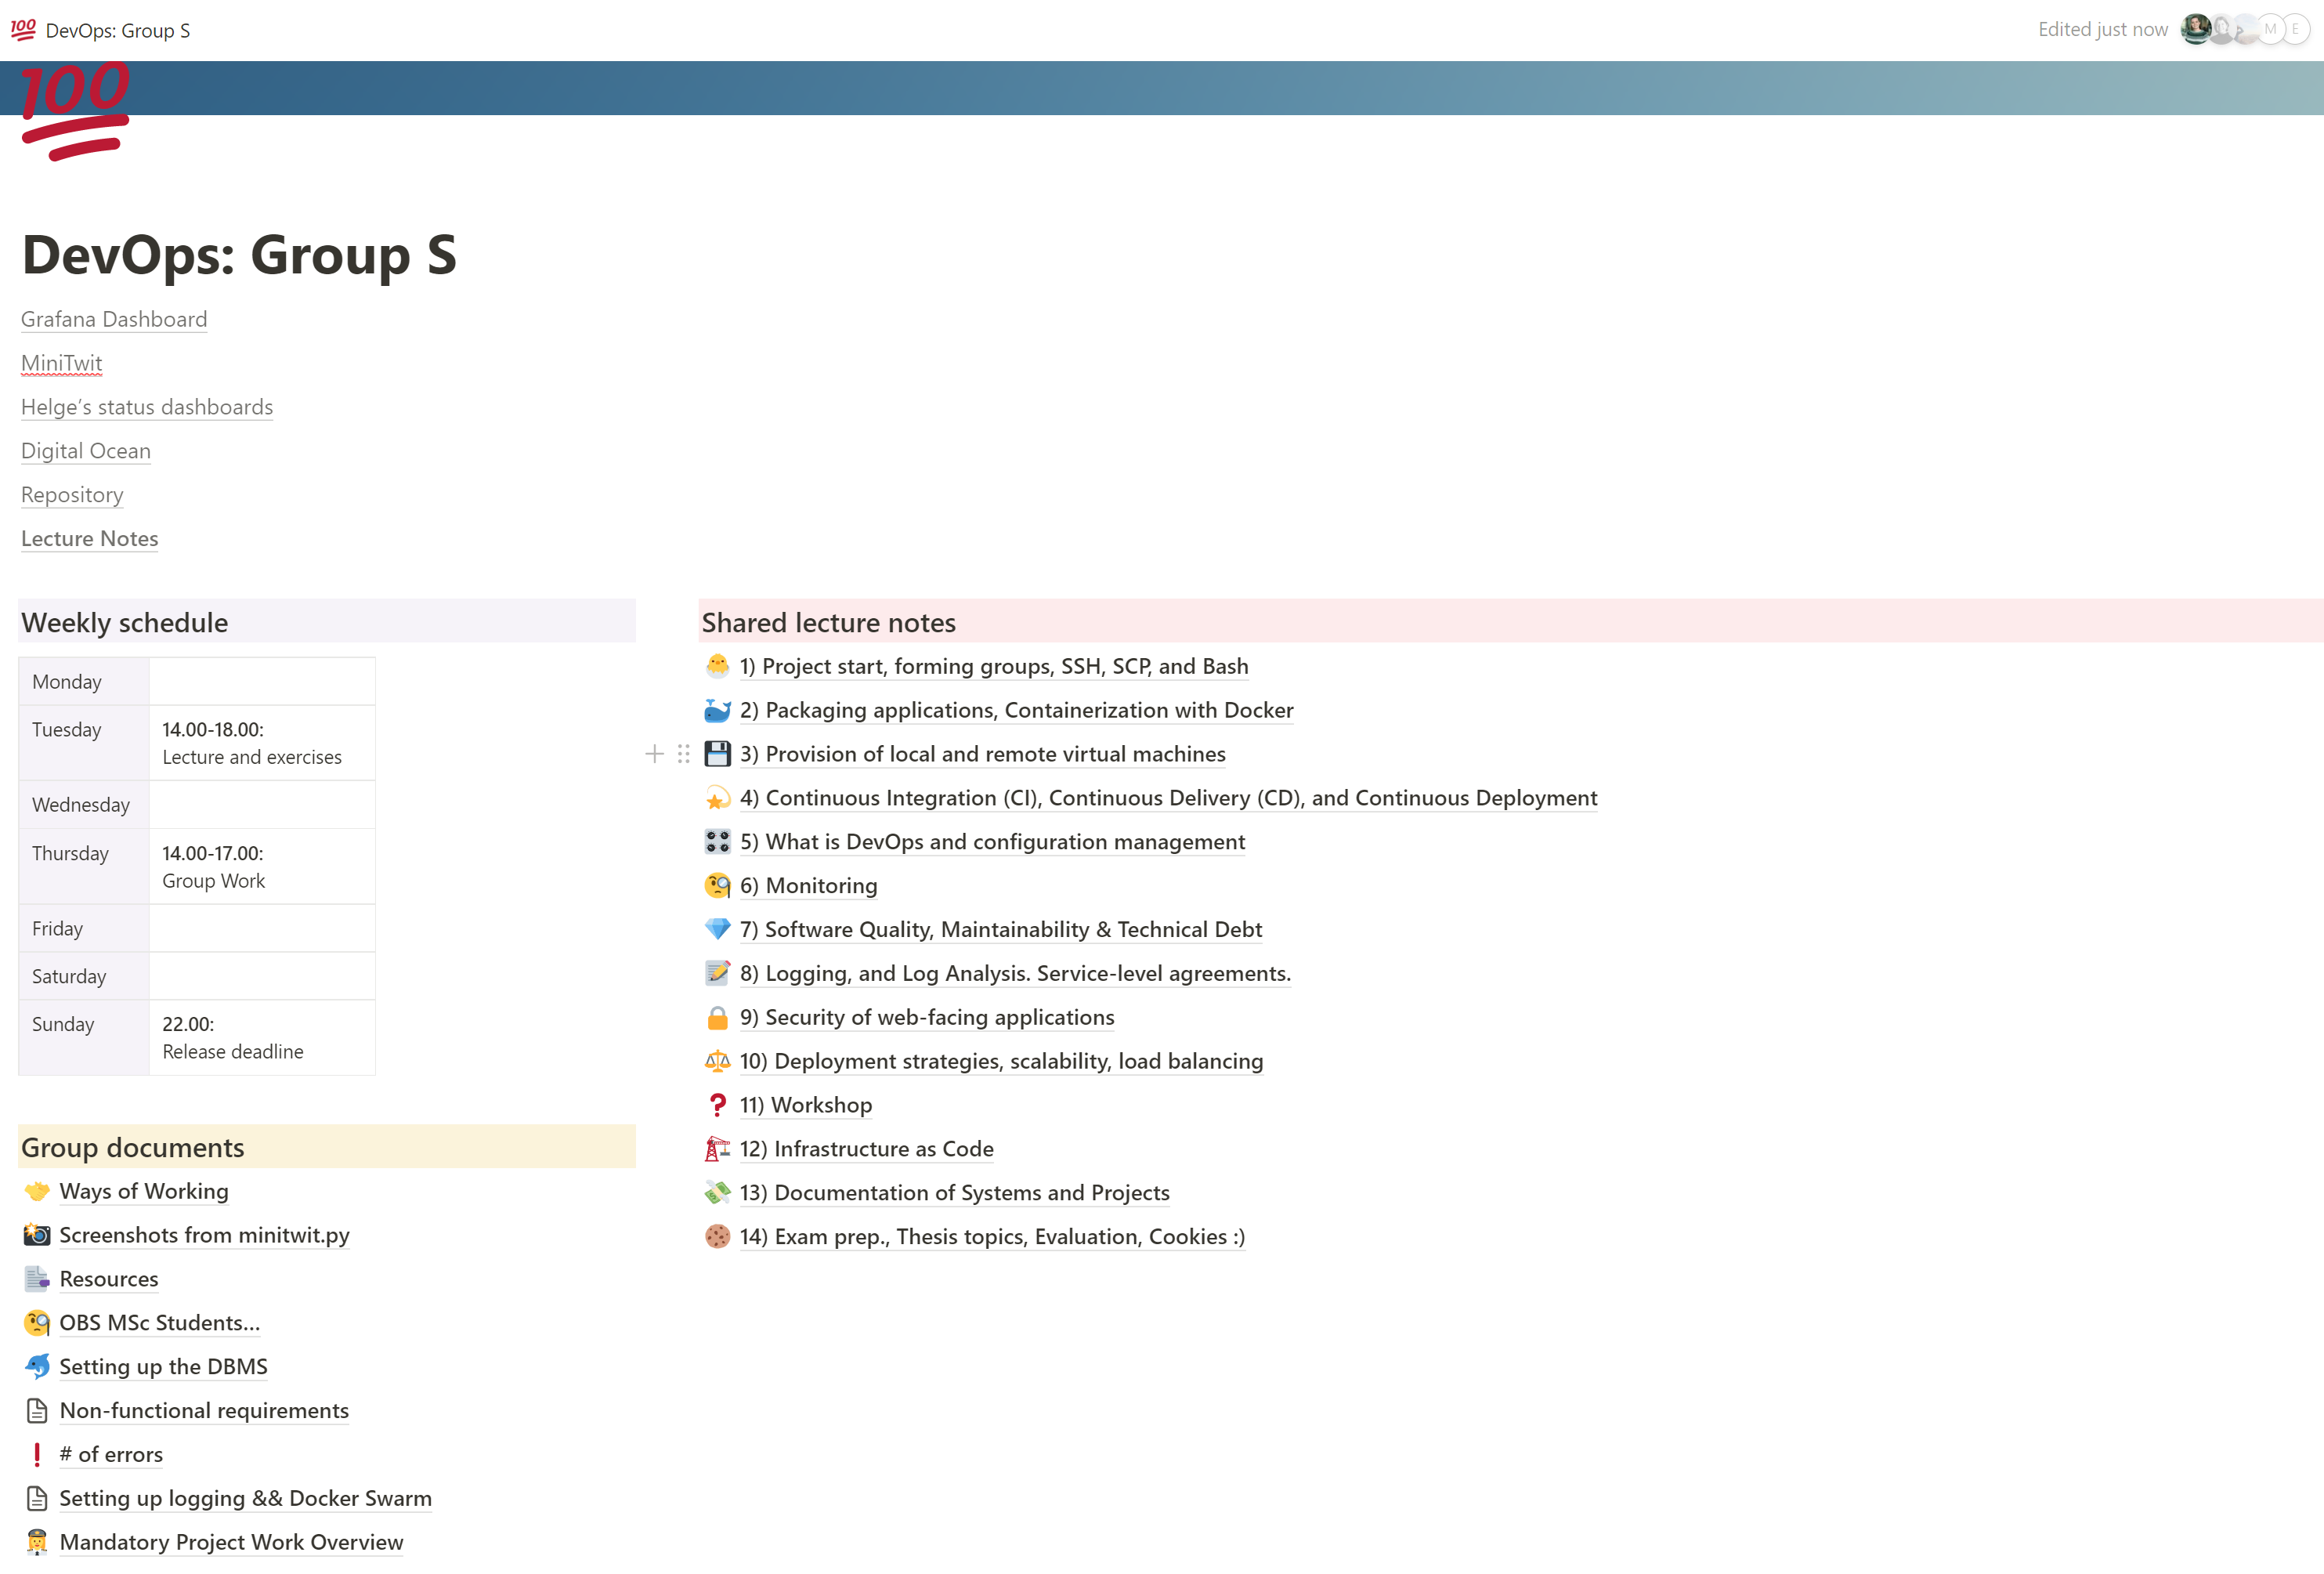
\includegraphics[width=.85\linewidth]{images/notion.png}
    \caption{Shared Notion.}
    \label{fig:notion}
\end{figure}

In addition to storing our MiniTwit repository, which will be further explained in the next section, we also used \textit{Github} for organizing tasks. Every Tuesday, following the lecture, we divided the tasks for the current week into subtasks on a Kanban board in our GitHub project and prioritized the new tasks in comparison to uncompleted tasks from the previous weeks. The board was consistently updated throughout the project with new task assignments and overall task progress, see Figure \ref{fig:kanban}. We used the Backlog-column for every unprioritized task, and the Todo column for the prioritized task the given week. 

\begin{figure}[H]
    \centering
    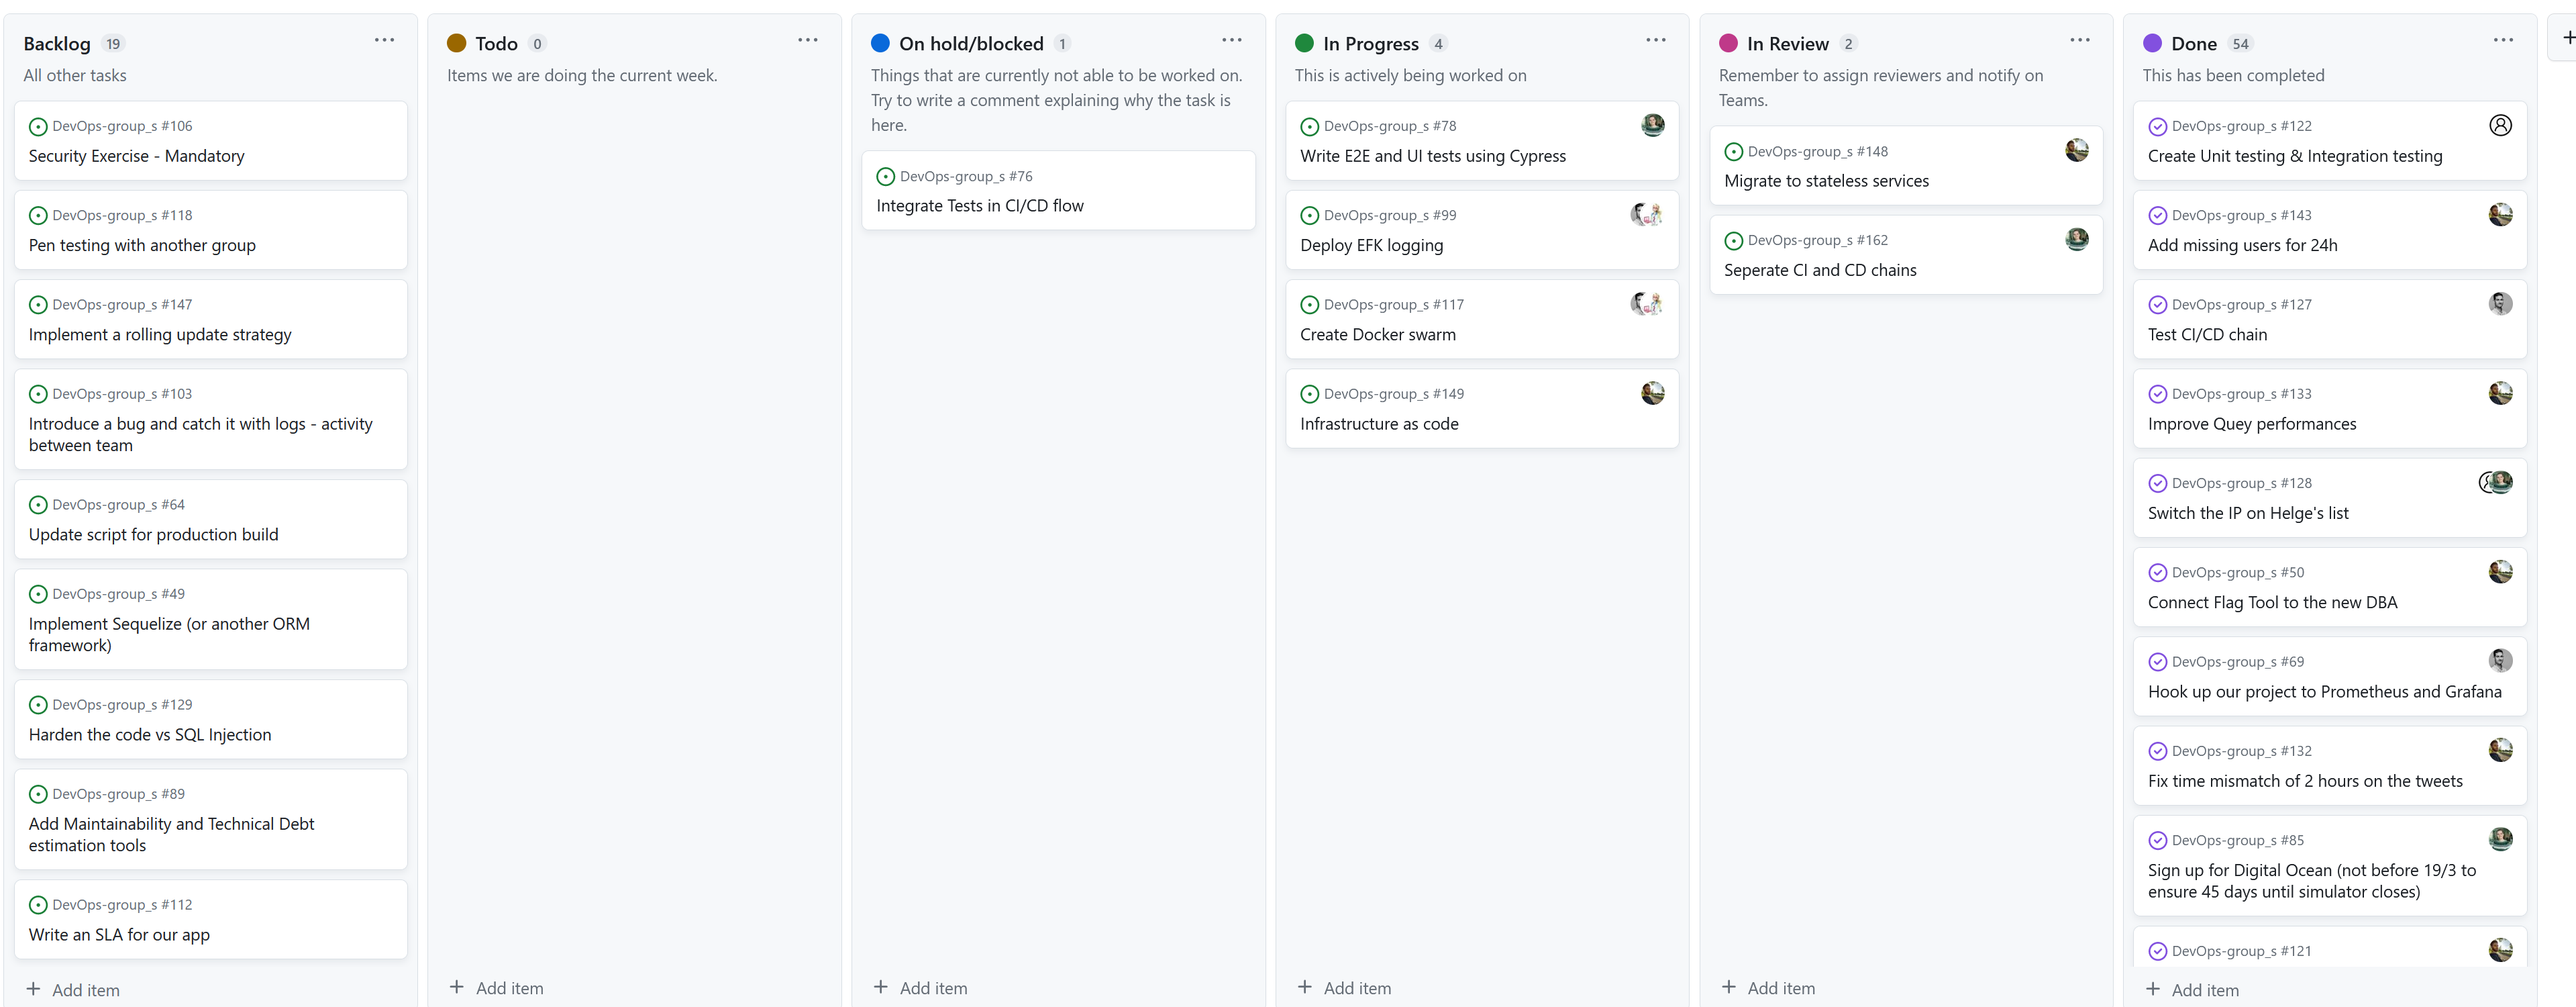
\includegraphics[width=\linewidth]{images/kanban.png}
    \caption{Our Kanban board}
    \label{fig:kanban}
\end{figure}

\subsubsection{Branching strategy}

Our team has implemented the Github Flow \cite{github_flow} branching strategy, which has one central \texttt{main} branch. To add new features, we start by checking out the \texttt{main} branch and push working changes to this local feature branch. Once the development work is completed, we create a pull request. Each pull request undergoes checks for merge conflicts, triggers our continuous integration (CI) pipeline, and requires review by at least one other team member.\\

The primary benefit of this approach lies in its simplicity. However, it also requires thorough checking and testing since it relies on a single central main branch. Our experience with this approach has highlighted certain challenges. Specifically, since we only added tests and separated our CI/CD chains relatively late in the process, we encountered issues with having to roll back \texttt{main}. This was due to only operating with a continuous deployment configuration which was triggered when changes were pushed to \texttt{main}.  

\subsection{CI/CD chains} 

%A complete description of stages and tools included in the CI/CD chains.
%That is, including deployment and release of your systems.

% OBS MSc students: Remember to log and provide good arguments for the choice of CI/CD system, i.e., why do you choose your solution instead of any other?

\subsubsection{Continuous Integration}

Our CI chain, see Figure \ref{fig:ci}, is triggered when a pull request is created. Note that the cypress testing step is grayed out since it was not thoroughly tested in the CI chain before we suspended our application. The diamond shapes are added to indicate where the chain can stop if a step fails. We intend to test and integrate this properly before the exam.\\ 

\noindent The CI chain has four main functionalities:

\begin{enumerate}
    \item Check out code 
    \item Login to Docker Hub
    \item Test the application
    \item Build and push images
\end{enumerate}

Due to time prioritization, we were unable to incorporate static checks into our CI chain. However, if we had implemented static checks, such as code analysis and linters, they would have been included before testing our application. By integrating these checks before testing, we avoid running unnecessary testing on an application that would fail either way. The same principle is the reasoning behind having testing before building and pushing our images.

% to edit: https://app.diagrams.net/#G1GlXy0XzENH587gelZ-4iOpl59S6CnzSF
\begin{figure}[H]
    \centering
    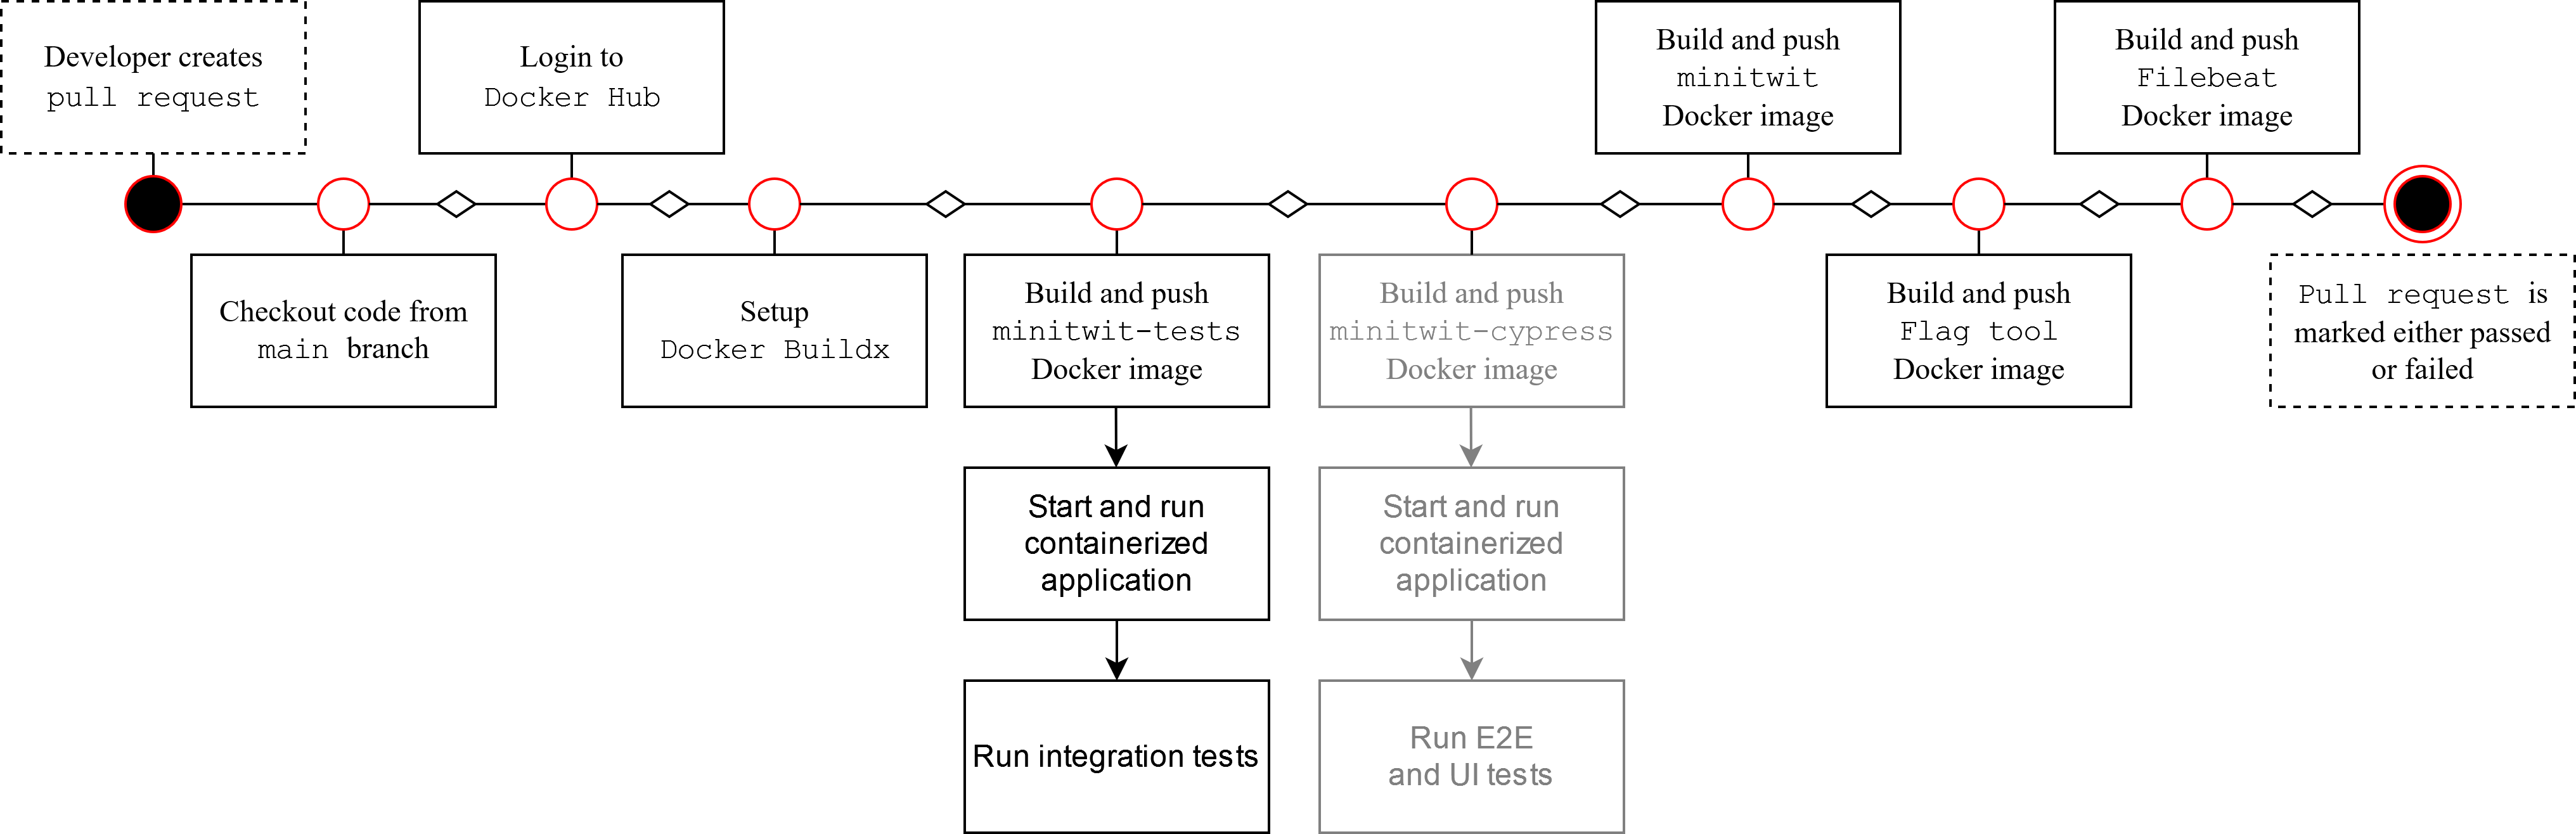
\includegraphics[width=\linewidth]{images/ci-flow.png} 
    \caption{Continous Integration flow diagram.}
    \label{fig:ci}
\end{figure}

In summary, our approach is to complete all necessary steps before deploying the code to our DigitalOcean servers. As part of our CI chain, we have chosen to include the creation and pushing of Docker images instead of placing them in the CD chain. Although these steps often belong in the CD chain, this decision allows us to proactively identify any issues associated with building or packaging the application into Docker images before merging to the main branch. Having limited experience working with Docker images, this approach favours a thorough understanding of Docker systems and documentation in case any issue arise within the images.

\subsubsection{Continuous Deployment}

\noindent Our CD chain, see figure \ref{fig:cd}, has two responsibilities: 

\begin{enumerate}
    \item Making the SSH connection available as an environment variable for the subsequent step in the deployment process
    \item Establishing an SSH connection to the remote server and executing the \texttt{deploy.sh} script
\end{enumerate}

% to edit: https://app.diagrams.net/#G1GlXy0XzENH587gelZ-4iOpl59S6CnzSF (see different tabs) 
\begin{figure}[H]
    \centering
    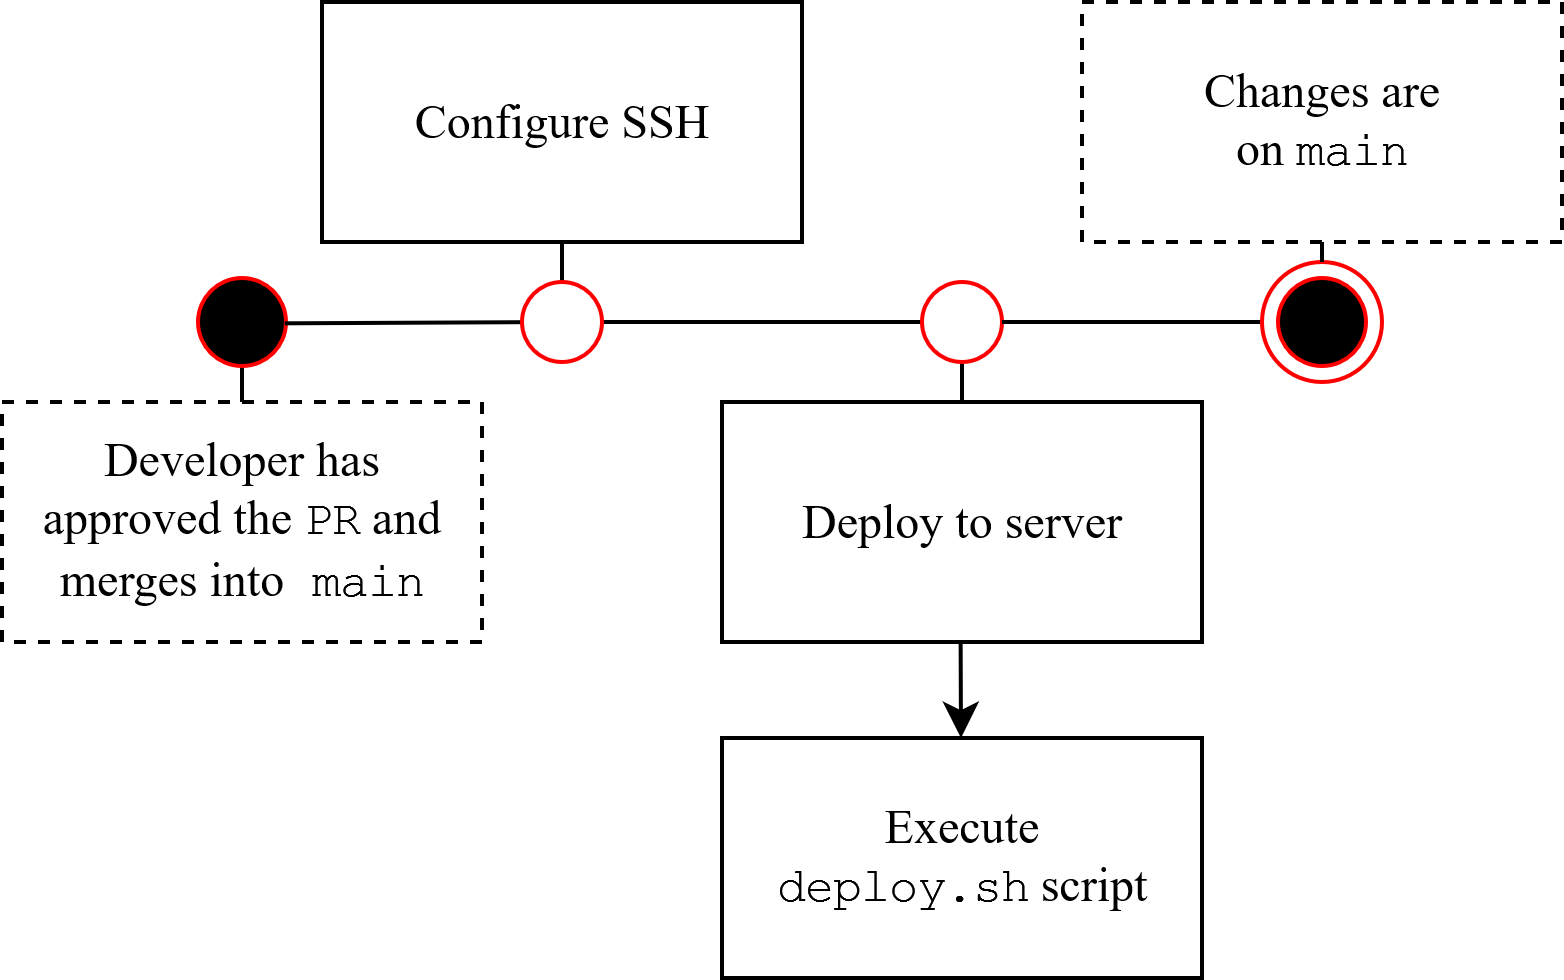
\includegraphics[width=.35\linewidth]{images/cd-flow.png} 
    \caption{Continous Deployment flow diagram.}
    \label{fig:cd}
\end{figure}

We did not manage to implement continuous delivery in the form of automatic releases or rolling updates in our CD chain.\\

When we fully implement using Terraform and enforce infrastructure-as-code, our CD chain will be deprecated. Instead of connecting to our CI/CD droplet and executing the deploy script, we will connect to our DO account via their API. Once connected, Terraform will take the lead in provisioning the resources specified in our repository configuration files. This includes creating or removing VMs, networks, IPs, and other defined components.

\subsection{Repository setup}

%Organization of your repositor(ies).
%That is, either the structure of mono-repository or organization of artifacts across repositories.
%In essence, it has to be clear what is stored where and why.

We chose a mono-repository setup containing the whole project. In the root folder, we have all relevant configuration files as well as sub-folders for every aspect of the system: the application source code, monitoring, and CI/CD pipeline. 

\begin{figure}[H]
    \centering
    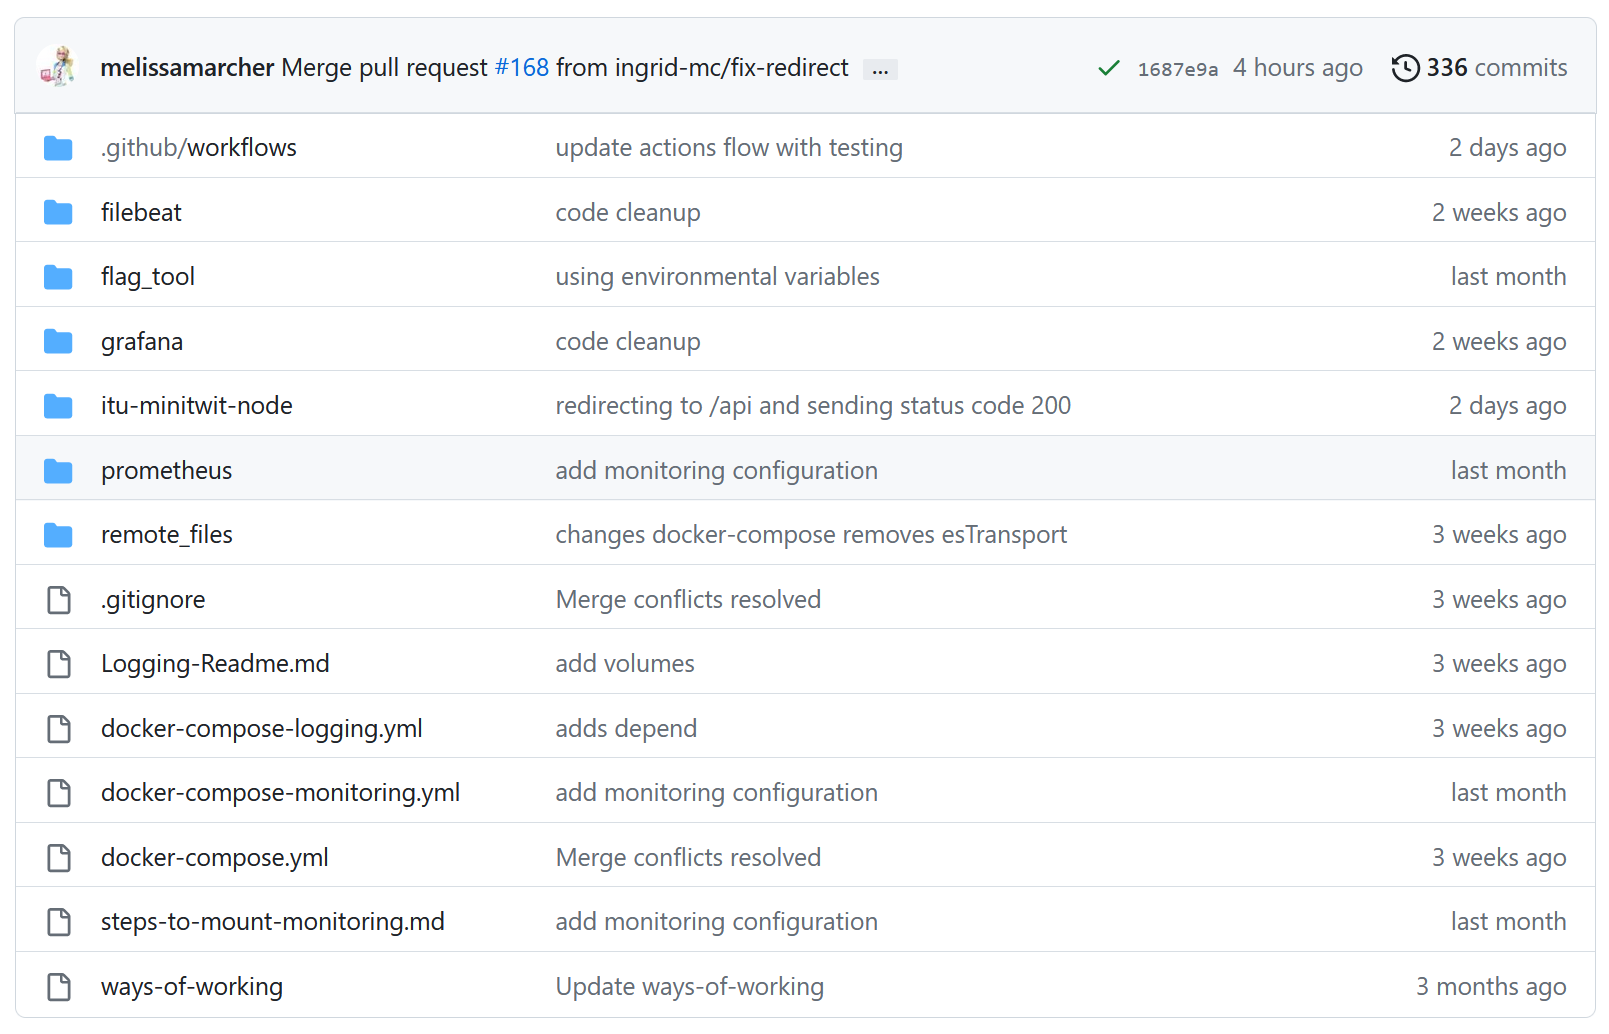
\includegraphics[width=.85\linewidth]{images/repo.png}
    \caption{\texttt{root} folder in our repository}
    \label{fig:repo}
\end{figure}

In the \texttt{itu-minitwit-node} folder, see Figure \ref{fig:minitwit-node}, we have our source code, tests, and Docker files. The \texttt{src} folder is further split into relevant subsystems such as database and entity handling, frontend in \texttt{views}, and routing between pages, see Figure \ref{fig:src} for a full overview.   

\begin{figure}[H]
    \centering
    \begin{minipage}{0.45\textwidth}
        \centering
        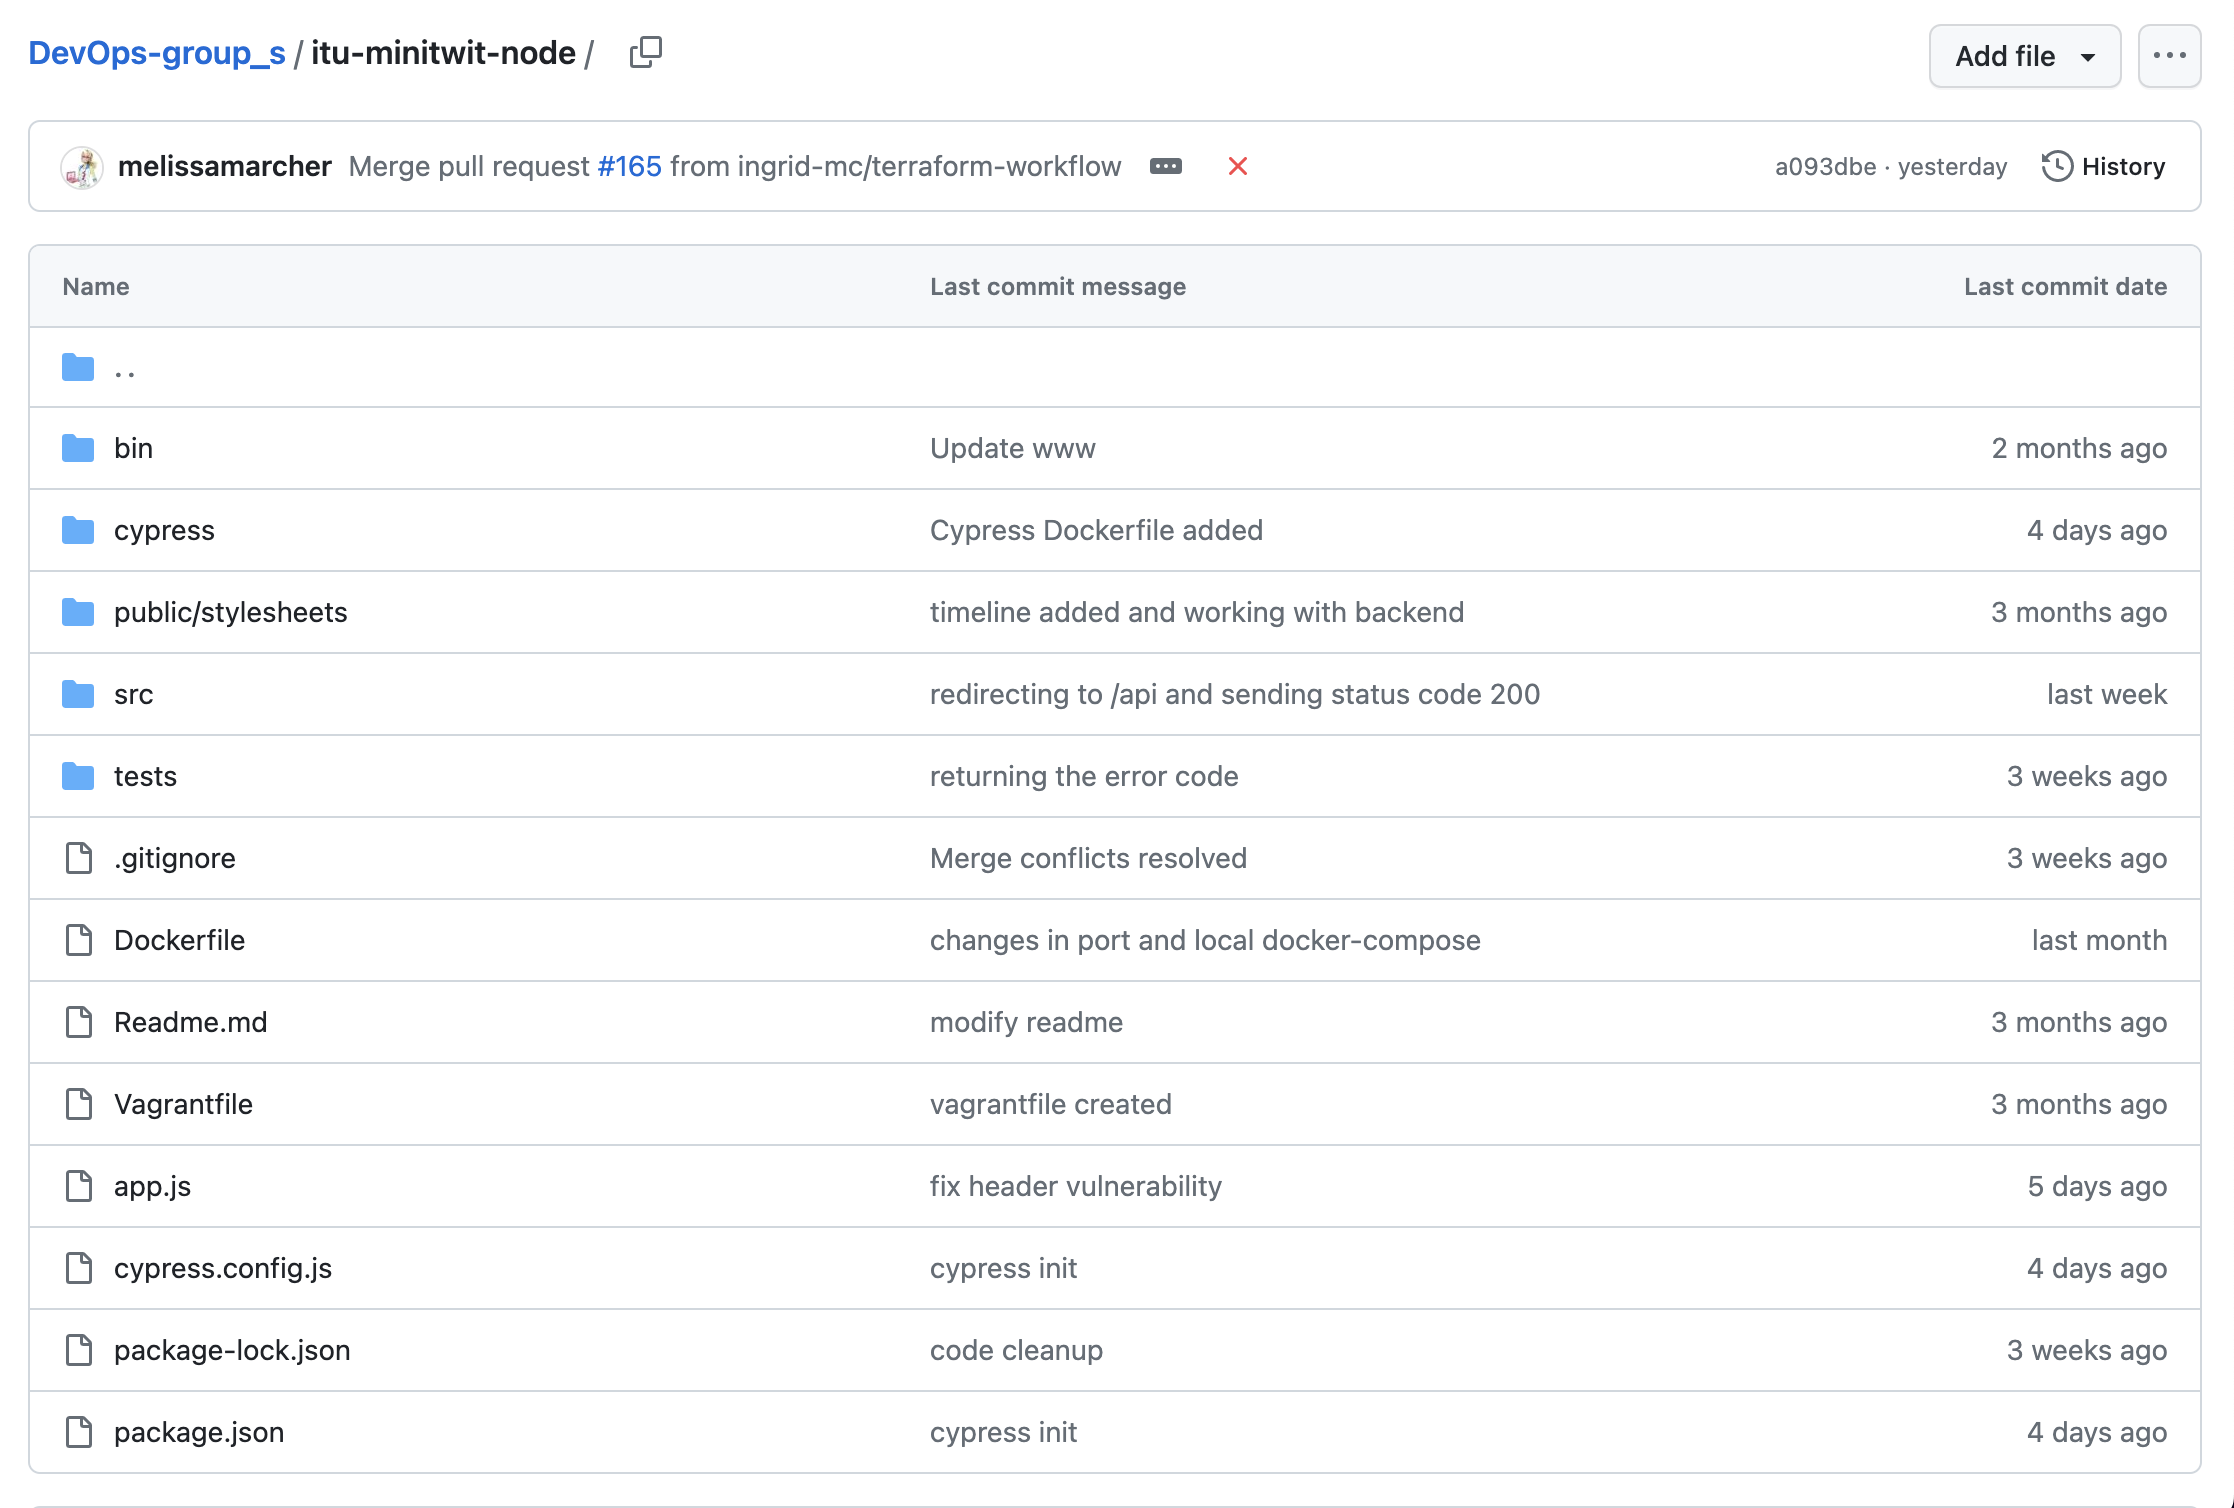
\includegraphics[width=1.15\textwidth]{images/itu-minitwit-node-folder.png}
        \caption{\texttt{itu-minitwit-node} folder}
        \label{fig:minitwit-node}
    \end{minipage}\hfill
    \begin{minipage}{0.45\textwidth}
        \centering
        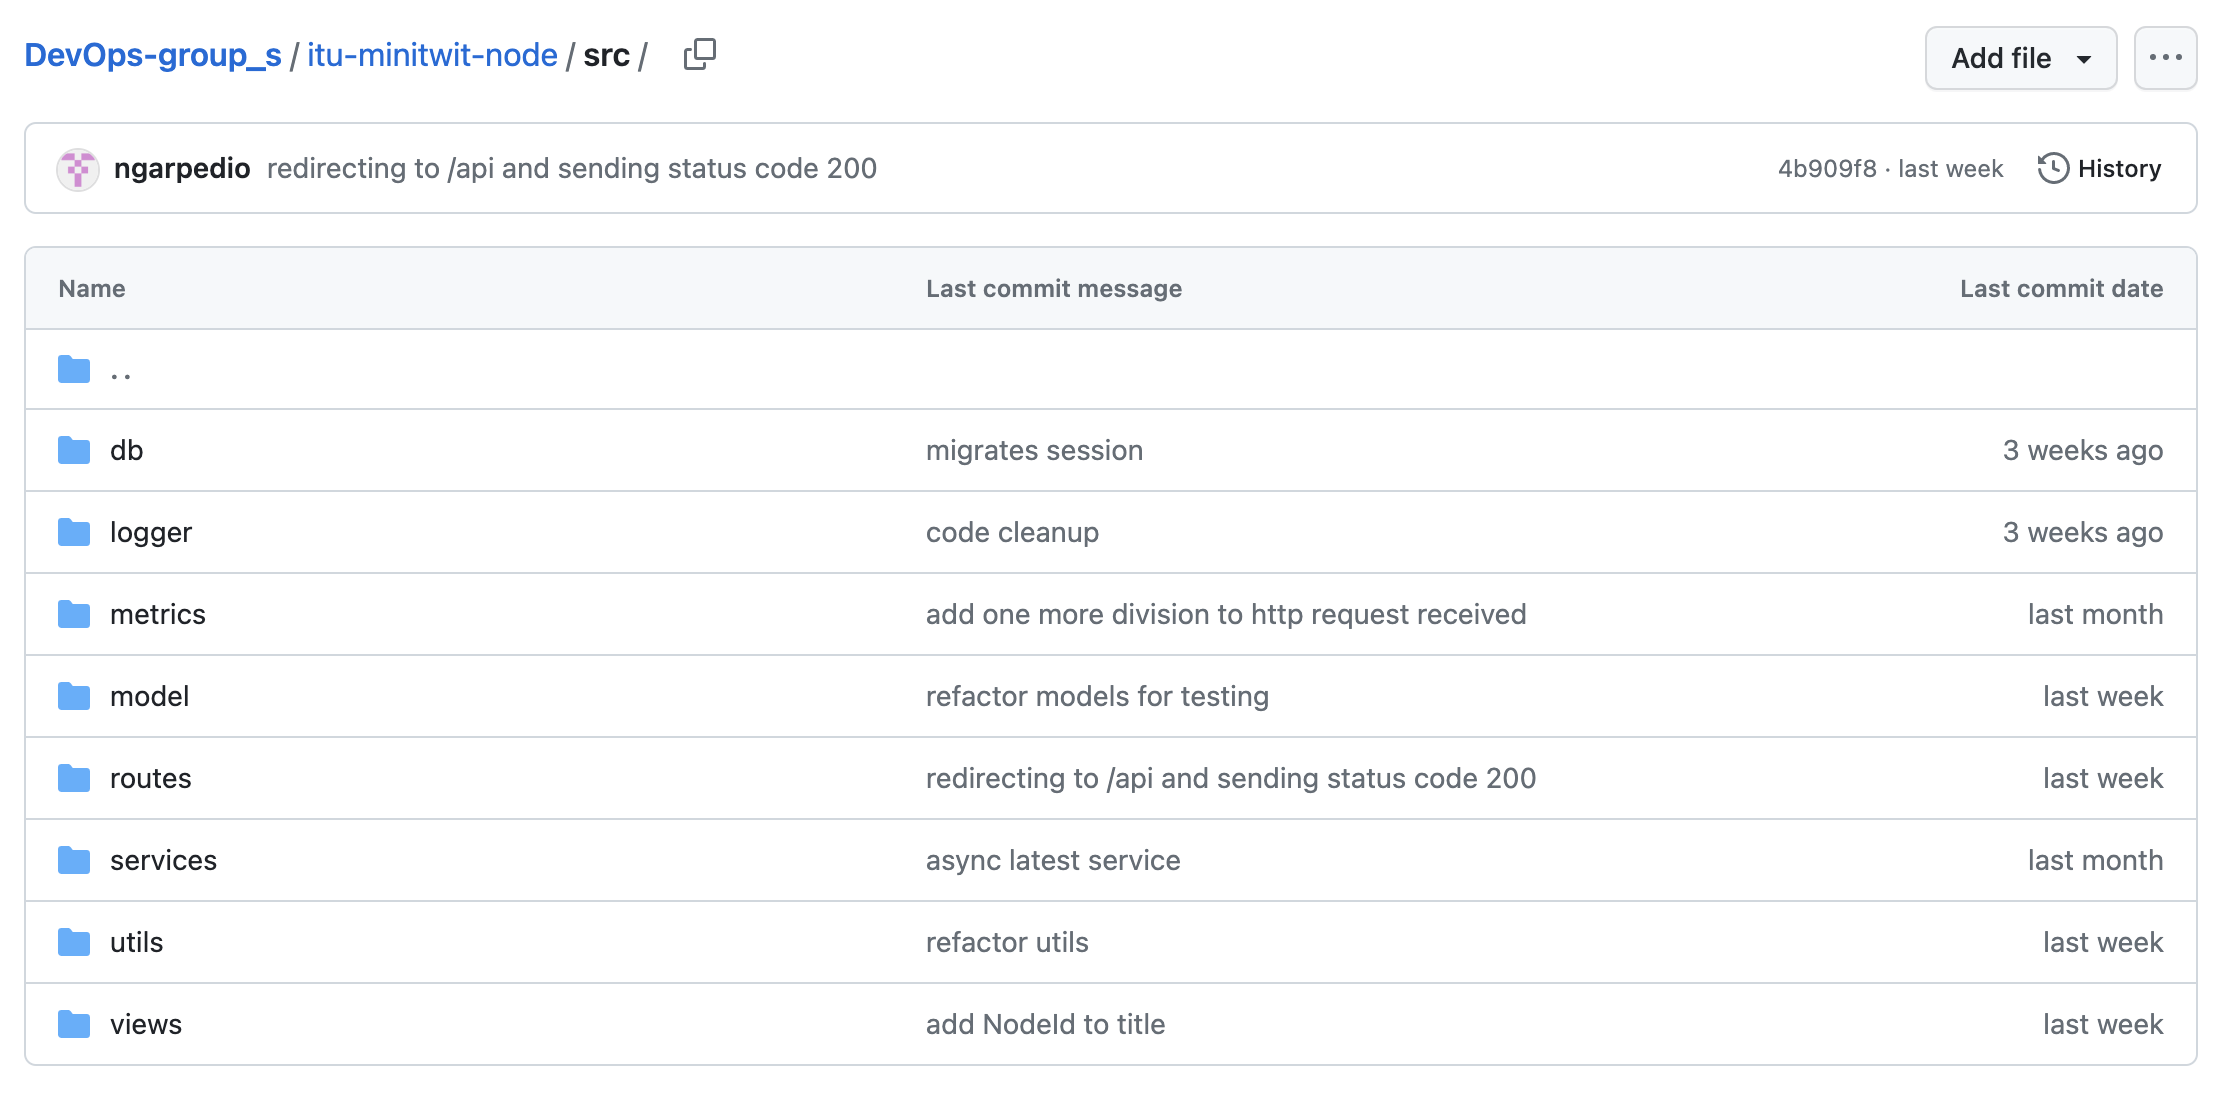
\includegraphics[width=1.15\textwidth]{images/src-folder.png} 
        \caption{\texttt{src} folder}
        \label{fig:src}
    \end{minipage}
\end{figure}

\subsection{Monitoring and logging}

\subsubsection{Monitoring}
In order to monitor our system we implemented a white box pull-based monitoring. Our implementation is rather reactive, as most of our metrics focus on the availability of our services and the infrastructure. However, we also do measure a few metrics, which give us insights into the software quality that we offer to our users. \\

In order to monitor our application and infrastructure we used Prometheus and Grafana. Prometheus is a monitoring system that scrapes our monitoring metrics every 15 seconds. The infrastructure monitoring metrics include the status of our Minitwit application and database, the uptime of the deployed containers, and memory usage. The application monitoring metrics consist of tracking the total count of HTTP errors and the error counts per individual endpoints, the number of active requests over time, and the response time of each endpoint. To collect those metrics, we instrumented our code with the \texttt{prom-client}, a Prometheus client library for Node.js applications. Grafana is a visualization web application, that was used to visualize gathered metrics in organized dashboards.

\subsubsection{Logging}
We chose to implement an EFK stack and use the Winston logging library \cite{winston} in combination with an ECSFormat module to log every HTTP request. We sort the messages based on their error level and write them into corresponding files. The log files are then continuously checked by Filebeat, which takes new entries and ships them to ElasticSearch where they are stored. Lastly, we use Kibana to query and visualize the data.\\

To test that our logging implementation works, we simulated a faulty sign-up request. We proceeded by sending a \texttt{/POST request} without providing any password value in the body. An \texttt{[ERR\_INVALID\_ARG\_TYPE]} error was logged, indicating that the implementation was working. A postmortem report of the incident has been written and added to the repository. The error can also be seen in Kibana, see Figure \ref{fig:kibana-bug}.

\begin{figure}[H]
    \centering
    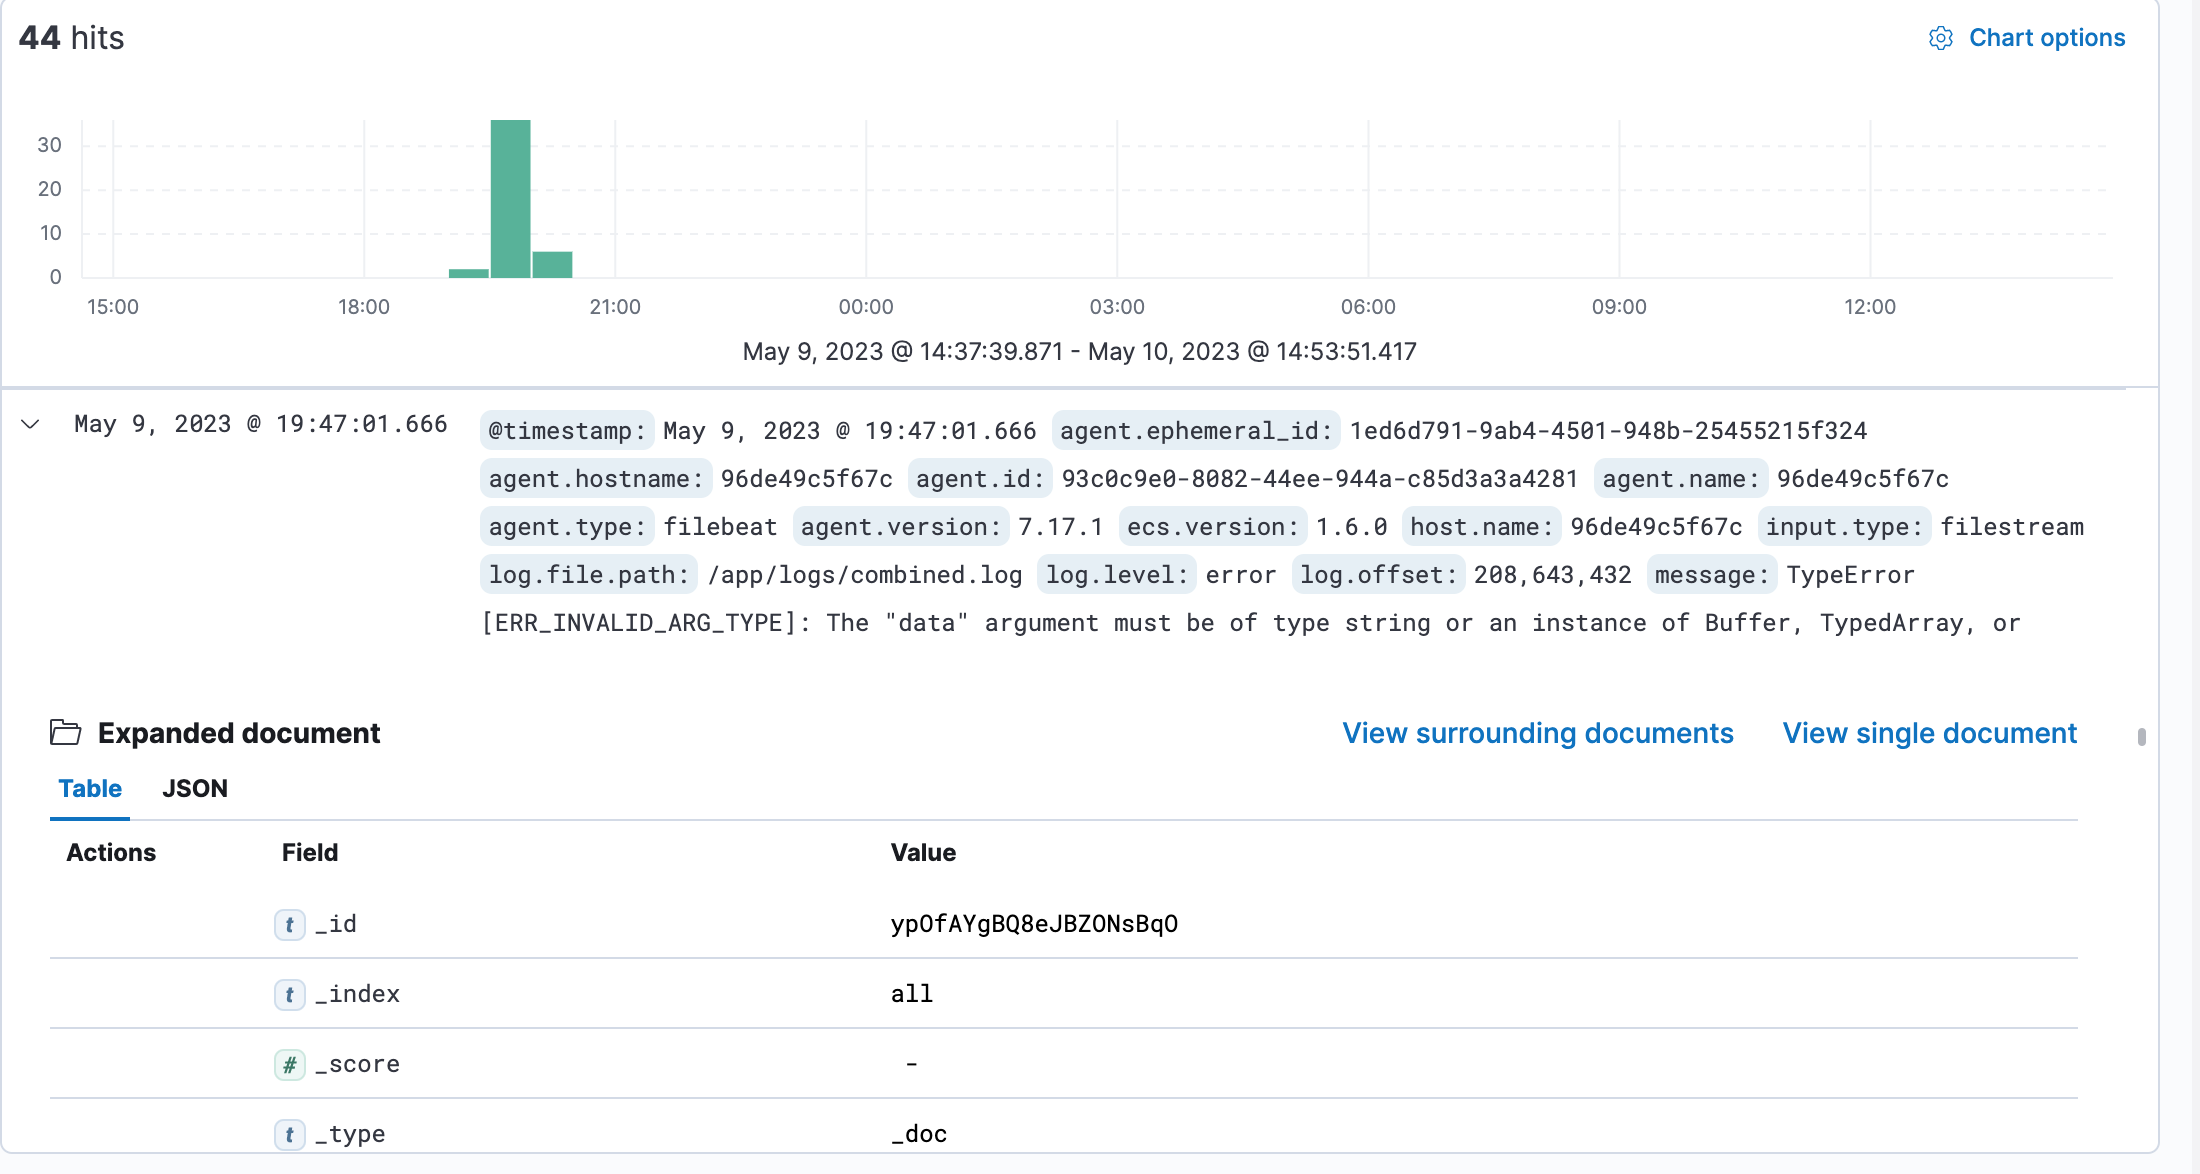
\includegraphics[width=\linewidth]{images/kibana-bug.png} 
    \caption{Error display in Kibana}
    \label{fig:kibana-bug}
\end{figure}

%Brief results of the security assessment.
\subsection{Security assessment}

\subsubsection{Risk identification}

The following assets have been identified and considered when making the security assessment:

\begin{itemize}
    \item User data: We store sensitive user information, such as emails and passwords
    \item Source code: The entire codebase of MiniTwit
    \item Production VMs: The servers utilized for running the MiniTwit application
    \item Logging data: Logs could potentially be misused to exploit the system
    \item Employees: Employee knowledge regarding the system and access credentials to various platforms
\end{itemize}

Based on the assets, we have composed seven security breach scenarios. For each scenario, the potential impact has been described and they have been categorized in terms of the three characteristics of security as defined in the CIA triad: Confidentiality, Integrity, and Availability\cite{bass2003software}. 

\begin{multicols}{2}
\begin{enumerate}

    \item \textbf{Third-party software contains malicious code or vulnerabilities}\\
    \textit{Impact:} Software vulnerabilities, data leaks \\ 
    \textit{Principle:} Integrity\\

    \item \textbf{Denial-of-service/distributed-denial-of-service attack}\\
    \textit{Impact:} Slowing down or bringing down systems \\ 
    \textit{Principle:} Availability\\

    \item \textbf{Brute-force attack}\\
    \textit{Impact:} Unauthorized access to user accounts, data leaks, manipulation of data \\
    \textit{Principle:} Confidentiality\\

    \item \textbf{SQL-injections}\\
    \textit{Impact:} Altering and/or destruction of data \\
    \textit{Principle:} Integrity

    \columnbreak
    
    \item \textbf{Man-in-the-middle attack (non-encrypted traffic)}\\
    \textit{Impact:} Data leaks \\
    \textit{Principle:} Integrity\\

    \item \textbf{Social engineering, ex. phishing e-mails}
    \textit{Impact:} Leak of company secrets, Leak of source code \\
    \textit{Principle:} Integrity\\

    \item \textbf{Attackers gain access to production VMs}\\
    \textit{Impact:} Unauthorized access, data leaks, bringing down systems \\
    \textit{Principle:} Integrity, Confidentiality,\\ Availability\\

\end{enumerate}
\end{multicols}

\subsubsection{Risk analysis and mitigation}

To determine the severity of each of the threats, we have placed them in a risk matrix to prioritize appropriate mitigation strategies. The severity categories are defined as: 
\begin{itemize}
    \item \textit{Insignificant:} Little to no impact 
    \item \textit{Marginal:} Manageable impact 
    \item \textit{Critical:} Difficult to recover
\end{itemize}

% edit figure here: https://docs.google.com/spreadsheets/d/1ZbBqvNd7IwXnbr_XMPb_ZFBBh0VcDOr2BV_DMQ8cIYg/edit?usp=sharing 
\begin{figure}[H]
    \centering
    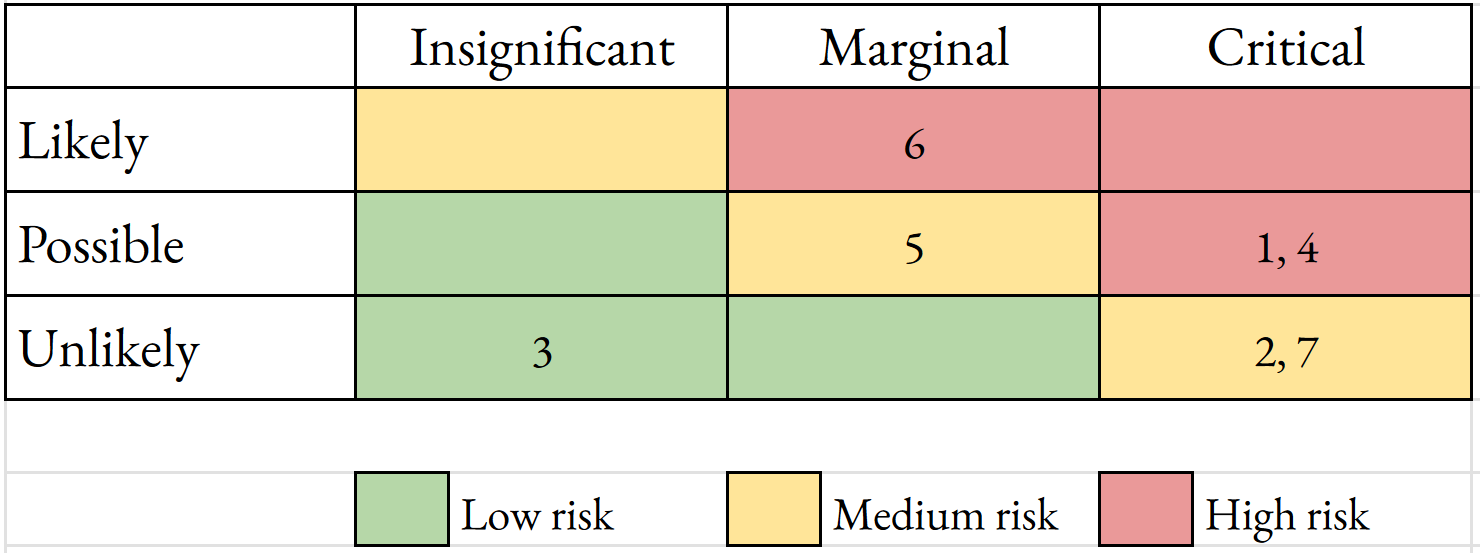
\includegraphics[width=.5\linewidth]{images/risk-matrix.png}
    \caption{Risk matrix with ids of threats.}
    \label{fig:risk}
\end{figure}


\noindent \textbf{High risk}\\
\indent \textbf{1)} The impact of a third-party vulnerability can vary broadly. Fortunately, this risk is also easy to mitigate, as static checks such as Snyk \cite{snyk} are able to identify which third-party libraries should be updated or removed.\\ 

\textbf{4)} In the worst case, SQL injections can destroy whole databases. the way we mitigated this risk was to implement an ORM framework, which abstracts away pure SQL from the source code. Further, it is possible to get automatic regular backups on your managed database in DigitalOcean.\\ 
    
\textbf{6)} This type of attack has many forms, is one of the most common, and can be almost impossible to mitigate fully. However, awareness of the potential dangers of phishing e-mails, unknown USB keys, etc. among employees is vital.\\  

\noindent \textbf{Medium risk}\\
\indent \textbf{2)} A distributed denial-of-service attack (DDoS) can bring down a system. Since it is distributed, it can be hard to detect. DigitalOcean takes some precautions in protecting against reflective DDoS attacks \cite{ddos_digitalocean}. However, we have not implemented any additional precautions.\\  
    
\textbf{5)} This risk can be mitigated through the simple use of HTTPS encryption. Due to lack of time, however, this risk has not been mitigated in Minitwit.\\ 

\textbf{7)} DigitalOcean allows firewall rules that protect access to virtual machines. However, we have not enforced any additional rules that protect our VMs.\\

\noindent \textbf{Low risk}\\ 
\indent \textbf{3)} Currently, it is possible to guess a user's password through brute force. If we were to mitigate this risk, two-factor authentication could be implemented.

\subsubsection{Automatic vulnerability test}
To test for vulnerabilities in our system, we used the tool OWASP ZAP \cite{owasp_zap}. It takes a URL as input and scans the web app for vulnerabilities. ZAP found seven vulnerabilities in our system - four marked as "medium" risk, and three marked as "low" risk. The alerts can be seen in Figure \ref{fig:zap-alerts}.

\begin{figure}[H]
    \centering
    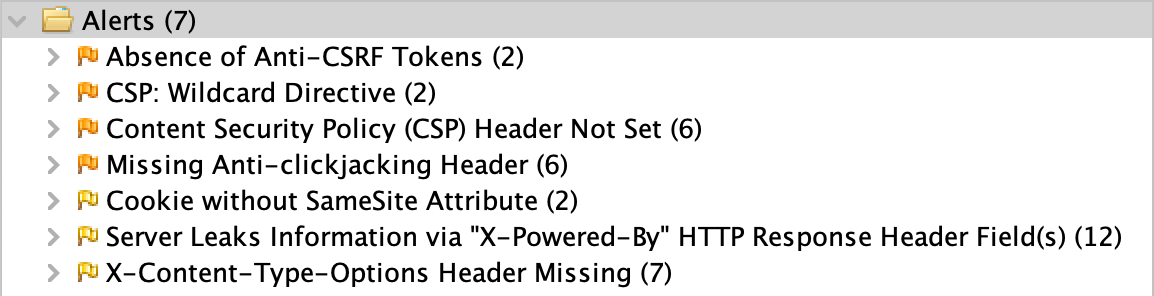
\includegraphics[width=.6\linewidth]{images/zap-alerts.png}
    \caption{The security alerts identified by OWASP ZAP.}
    \label{fig:zap-alerts}
\end{figure}

We decided to focus on the alert \textit{"Server Leaks Information via 'X-Powered-By' [...]"}. Here, ZAP tells us that frameworks used by our application will be visible in HTTP response headers. It means that attackers could potentially check for vulnerabilities in these frameworks and use them to their advantage. The 'X-Powered-By' field can easily be omitted by including the line "\texttt{app.disable('x-powered-by');}" in our \texttt{app.js} file. However, we decided to include the Helmet dependency \cite{helmet} instead, as it includes an array of response header protection, not just on the 'X-powered-by' field. We were able to see traces of the ZAP scan in our EFK stack, seen in Figure \ref{fig:kibana-logs-zap}, which shows a spike in activity for a few seconds (the scan was done after the simulator was shut down).

\begin{figure}[H]
    \centering
    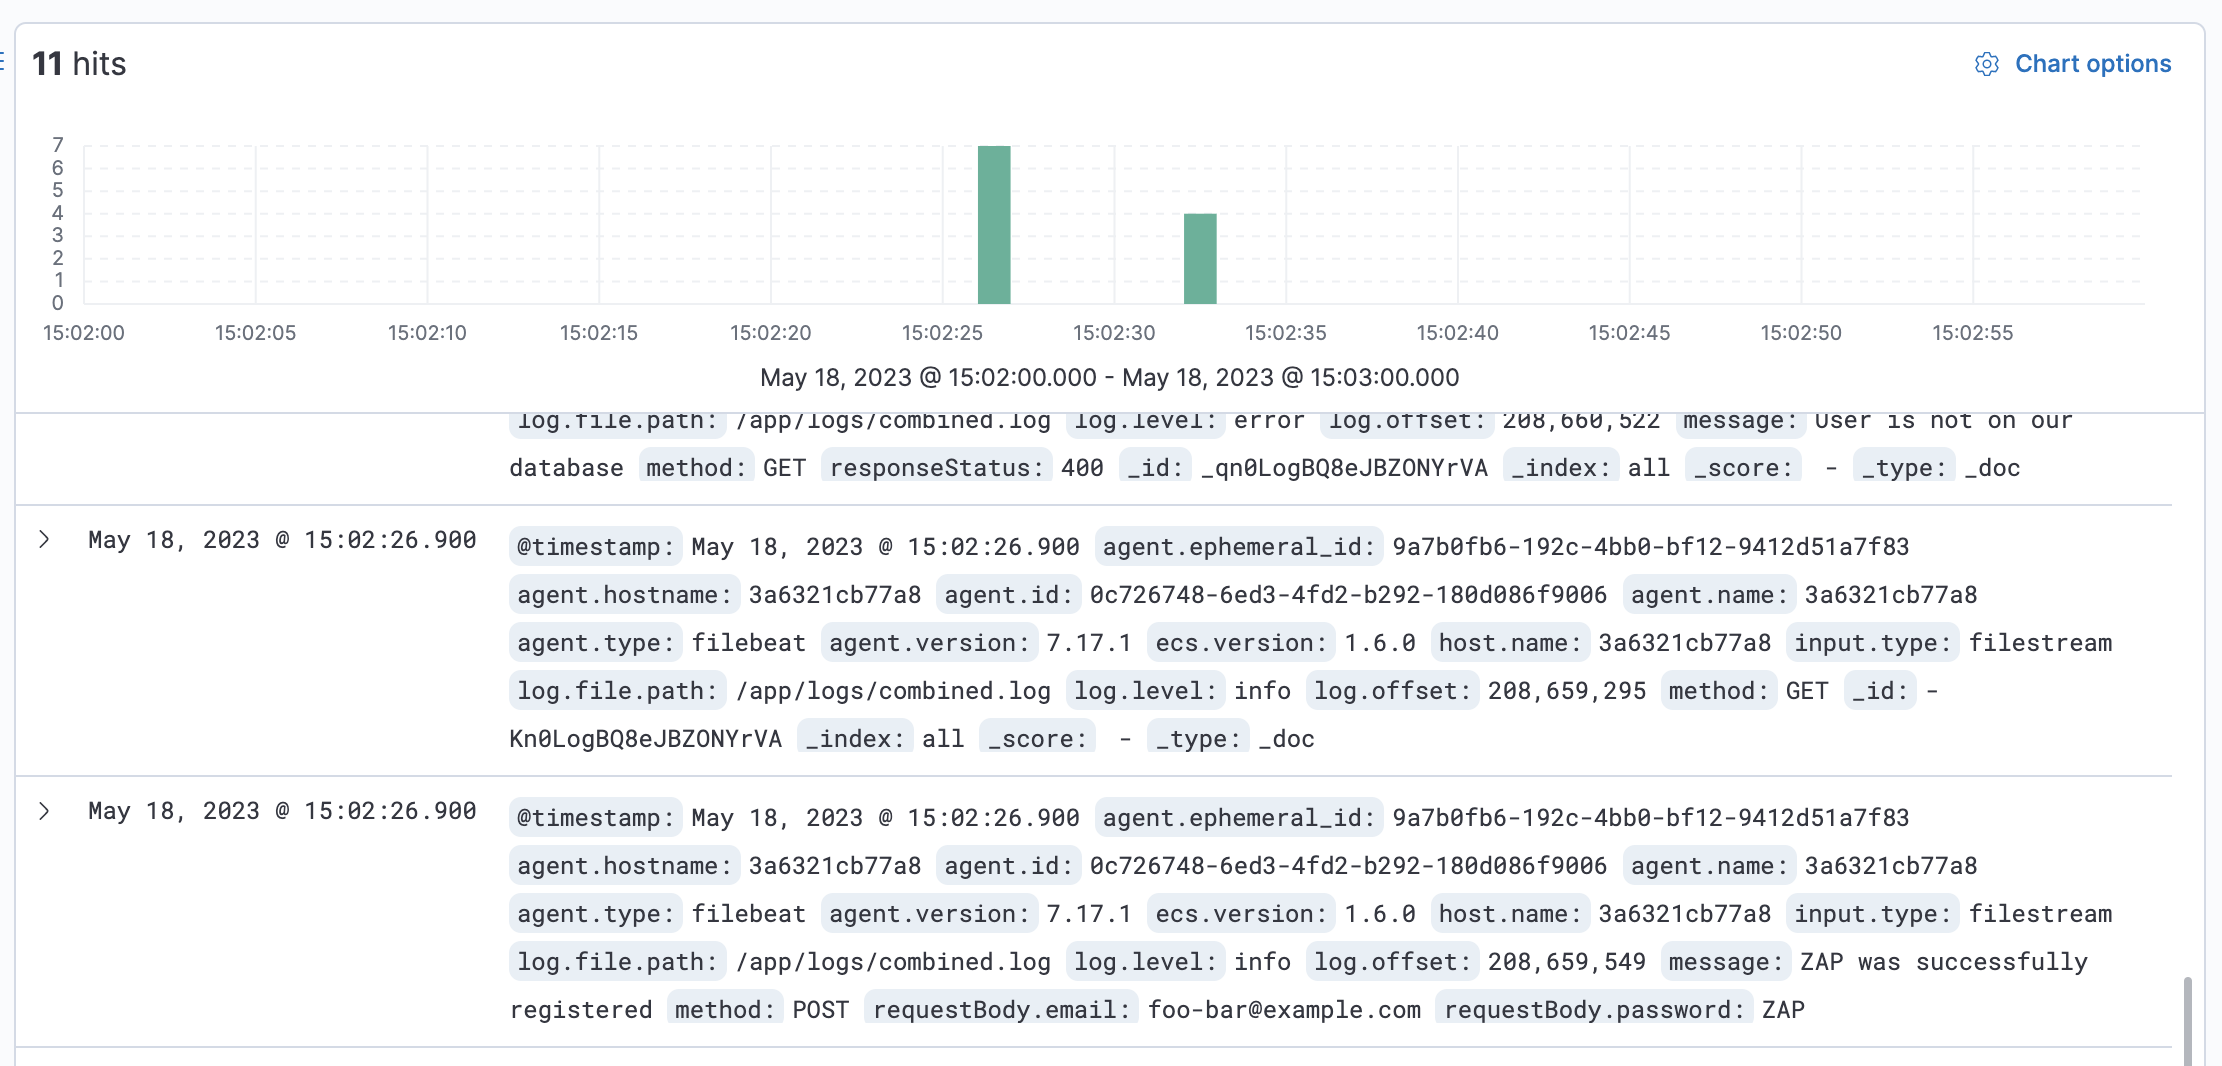
\includegraphics[width=\linewidth]{images/kibana-zap-logs.png}
    \caption{Activity in the logs after running a security scan with OWASP ZAP.}
    \label{fig:kibana-logs-zap}
\end{figure}

% What does the Zap test look like now?

We would have liked to run the OWASP ZAP check once again after including the Helmet dependency. However, we had to shut down the app before running ZAP again to avoid receiving a large bill from DigitalOcean. 


\subsection{Scaling and load balancing strategy}
%Applied strategy for scaling and load balancing.
\subsubsection{Scaling and Docker Swarm}
Although DigitalOcean makes it easy to scale applications vertically by increasing droplet size, we decided to scale our system horizontally using Docker Swarm \cite{docker_swarm}. We decided on Docker Swarm mode as it allows for container orchestration, which is something we wanted to get experience with. In addition, Docker Swarm includes capabilities like self-healing (restarting services when they are down) and built-in load balancing. The cluster is built in code using Terraform\cite{terraform}. The \texttt{main.tf} file sets up one leader (manager) droplet, one manager droplet, and two worker droplets in DigitalOcean. The \texttt{minitwit\_stack.yml} file sets up services for the cluster. All services are in replicated mode, with three replicas of \texttt{minitwit}, two replicas of \texttt{filebeat}, and a single \texttt{flagtool}. Here, we also add additional services: a Docker Swarm Visualizer and an NGINX load balancer. If we need to scale up the capacity of our application in the future, we can simply rewrite the Terraform file and redeploy it.

\subsubsection{Load balancing}
Adding an NGINX load balancer in our stack file means that we not only have load balancing between nodes but also "in front of" the whole cluster. While the NGINX load balancer distributes task load to an appropriate node, the ingress load balancer in each node makes sure that a request to a specific service will be rerouted to the node running that service. The current system does not use HTTPS for secure client-server communication. However, if we were to implement that in the future, an added bonus of having an extra load balancer is that only traffic to and from that load balancer would need to be secure, as all other communication would run within a closed system. 

\subsection{Use of AI-assistants}
We used two different AI assistants during the project: GitHub Copilot and ChatGPT. A few of the team members used GitHub Copilot as a code assistant. This speeds up the coding process, particularly during the initial phase of rewriting the application from Flask to Express.js. ChatGPT was used by all team members and used more as an occasional helper when stuck with a code or a configuration problem. Its effectiveness varied, occasionally leading to confusion. We observed that ChatGPT is more adept at providing general code structures rather than specific configurations. If ChatGPT was used for any sections of the report, we have mentioned it in the relevant section. 

%In case you have used AI assistants for writing code during your project or to write the report:
%Explain which system(s) you used during the project.
%Reflect on how it supported/hindered your process.
%In essence it has to be clear how code or other artifacts come from idea into the running system and everything that happens on the way.
